\section{Construction of ODE Model}
\label{sec:wo_detect}
We investigate the selfish detection in this and the following sections.
Specifically, in this section, the ordinary differential equation model
is constructed to capture the state change with time.
\subsection{Case 1: without detection}
\label{subsec:wo_detc}
\begin{figure}
  \centering
  {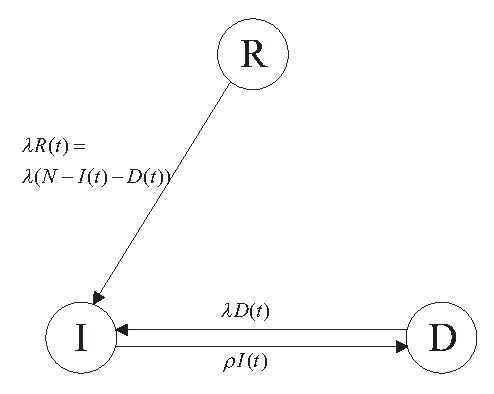
\includegraphics[width=0.25\textwidth]
  {fig/state_transition_no_detect.eps}}
     \caption{State transition of the relay nodes without detection.}
     \label{fig:ss_wo_dt}
\end{figure}
In the case without detection,
the relay node with message can become the selfish node,
but the selfish detection is not conducted.
Then the state transition is shown
in Fig.~\ref{fig:ss_wo_dt} with the following rules.
The nodes change from state $R$ to state $I$ if they contact $src$.
The corresponding incremental rate of state $I$ is $\lambda R(t)$ at time $t$.
The selfish node also may contact $src$ in the opportunistic network.
Then the total incremental rate of $I$ is
$\lambda (R(t)+D(t))=\lambda (N-I(t))$.
Additionally, the infected node may become the selfish node with rate $\rho$.
Thus we can obtain the derivative of $I(t)$ with respect to $t$,
\begin{small}
\begin{equation}
\nonumber
\begin{aligned}
\frac{\mathrm{d} I(t)}{\mathrm{d} t} &= \lambda (N-I(t)) - \rho I(t).
\end{aligned}
\end{equation}
\end{small}
where $\lambda$ and $\rho$ are constants.
Similar to $\frac{\mathrm{d} I(t)}{\mathrm{d} t}$,
we can get the change rate of state $D$ and state $R$,
i.e. $\frac{\mathrm{d} D(t)}{\mathrm{d} t}$ and
$\frac{\mathrm{d} R(t)}{\mathrm{d} t}$,
and obtain the model,
\begin{small}
\begin{equation}
\label{eq:IDR_wo}
\begin{aligned}
\frac{\mathrm{d} I(t)}{\mathrm{d} t} &=  \lambda (N-I(t)) - \rho I(t),\\
\frac{\mathrm{d} D(t)}{\mathrm{d} t} &= - \lambda D(t) + \rho I(t),\\
\frac{\mathrm{d} R(t)}{\mathrm{d} t} &= - \lambda (N-I(t)-D(t)).
\end{aligned}
\end{equation}
\end{small}
Since $I(t)$ in (\ref{eq:IDR_wo}) is formed by the first-order first-power
ordinary differential equations (ODE)~\cite{CC2007PerfAnaly},
we can calculate the general solutions of $I(t)$, that is,
\begin{small}
\begin{equation}
\nonumber
\begin{aligned}
I(t) = C_{I} e^{-(\lambda + \rho)t} + \frac{ \lambda N }{ \lambda + \rho }.
\end{aligned}
\end{equation}
\end{small}
Note that $I(0)=0$, $D(0)=0$ and $R(0)=N$,
which means only $src$ carries the message.
Thus $C_{I} = \frac{ -\lambda N }{ \lambda + \rho }$, and
\begin{small}
\begin{equation}
\nonumber
\begin{aligned}
I(t) = \frac{ \lambda N }{ \lambda + \rho }(1- e^{-(\lambda + \rho)t}),
\end{aligned}
\end{equation}
\end{small}
where $0 \le t \le T$.
Similarly, we can calculate the general solution of the first-order ODE $D(t)$
from $\frac{\mathrm{d} D(t)}{\mathrm{d} t} + \lambda D(t) = \rho I(t)$,
\begin{small}
\begin{equation}
\nonumber
\begin{aligned}
D(t) &= C_{D} e^{-\int \lambda dt} + e^{-\int \lambda dt} \int \rho I(t) e^{\int \lambda dt} dt \\
&= C_{D} e^{- \lambda t} +
e^{- \lambda t} \int \rho \frac{ \lambda N }{ \lambda + \rho } (1 - e^{-(\lambda + \rho)t}) e^{ \lambda t} dt \\
&= C_{D} e^{- \lambda t} + \frac{ \lambda N }{ \lambda + \rho } e^{-(\lambda + \rho)t} + \frac{ \rho N }{ \lambda + \rho }
\end{aligned}
\end{equation}
\end{small}
Because of $D(0)=0$,
\begin{small}
\begin{equation}
\nonumber
\begin{aligned}
D(t) &= -N e^{- \lambda t} + \frac{ \lambda N }{ \lambda + \rho } e^{-(\lambda + \rho)t} + \frac{ \rho N }{ \lambda + \rho }.
\end{aligned}
\end{equation}
\end{small}
Since $I(t)+D(t)+R(t)=N$, $0 \le t \le T$,
$R(t)$ can be computed based on the solved solution of $I(t)$ and $D(t)$.
Thus the solution of (\ref{eq:IDR_wo}) can be derived as
\begin{small}
\begin{equation}
\label{eq:IDR_wo_solu}
\begin{aligned}
I(t) &= \frac{ \lambda N }{ \lambda + \rho }(1- e^{-(\lambda + \rho)t}), \\
D(t) &= N (\frac{\lambda e^{-(\lambda + \rho)t} + \rho}{ \lambda + \rho } - e^{- \lambda t}), \\
R(t) &= N e^{- \lambda t},
\end{aligned}
\end{equation}
\end{small}
which depicts the change of the states when the time ranges from $0$ to $T$.
And $I(t)$, $D(t)$, $R(t)$ $\ge 0$ always hold when $t \le 0$.
From the solutions of $I(t)$, $D(t)$ and $R(t)$,
we can find that $I(t) \rightarrow \frac{ \lambda N }{ \lambda + \rho }$,
$D(t) \rightarrow \frac{ \rho N }{ \lambda + \rho }$,
and $R(t) \rightarrow 0$
when $t \rightarrow + \infty$.
To verify the validity of the ODE model (\ref{eq:IDR_wo}),
we conduct the simulations with randomly settings.
The corresponding results are presented in Section.~\ref{subsec:pe_valid}.

Note that $U(t)=0$, $\forall t$,
in the situation without detection.
The total cost $J$ in (\ref{eq:obj}) is determined by $D(t)$, $0 \le t \le T$,
which is the total wasted reward by the selfish behaviors.
Based on the calculated result in (\ref{eq:IDR_wo_solu}),
we can compute $J$ as
\begin{small}
\begin{equation}
\nonumber
\begin{aligned}
J &= \int_{0}^{T} (1-\alpha) D(t) dt, \\
&= \int_{0}^{T} (1-\alpha) N (\frac{\lambda e^{-(\lambda + \rho)t} + \rho}{ \lambda + \rho } - e^{- \lambda t}) dt, \\
&= N (1-\alpha) \left( \frac{\lambda (1-e^{-(\lambda+\rho)T})}{ (\lambda + \rho)^{2} }
+ \frac{\rho T}{\lambda + \rho}
- \frac{1-e^{-\lambda T}}{\lambda} \right).
\end{aligned}
\end{equation}
\end{small}
The total paid reward can be calculated as
\begin{small}
\begin{equation}
\nonumber
\begin{aligned}
P &= \beta \int_{0}^{T} I(t) + D(t) dt, \\
&= \beta \int_{0}^{T} (N - N e^{- \lambda t}) dt, \\
&= N \beta (T - \frac{ 1 - e^{-\lambda T} }{\lambda} ).
\end{aligned}
\end{equation}
\end{small}
Furthermore, the fraction between the wasted reward and the total paid reward is
\begin{small}
\begin{equation}
\nonumber
\begin{aligned}
\frac{\int_{0}^{T} D(t) dt}{\int_{0}^{T} I(t) + D(t) dt}
&= \frac{ \frac{\lambda (1-e^{-(\lambda+\rho)T})}{ (\lambda + \rho)^{2} }
+ \frac{\rho T}{\lambda + \rho}
- \frac{1-e^{-\lambda T}}{\lambda} }
{T - \frac{ 1 - e^{-\lambda T} }{\lambda} }.
\end{aligned}
\end{equation}
\end{small}

\subsection{Case 2: with full detection}
\label{subsec:full_detc}
\begin{figure}
  \centering
  {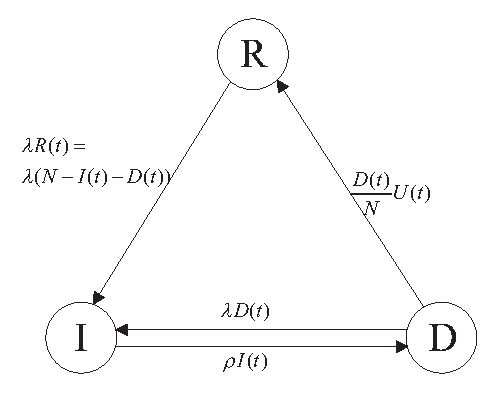
\includegraphics[width=0.25\textwidth]
  {fig/state_transition_detect.eps}}
     \caption{State transition of the relay nodes.}
     \label{fig:ss_dt}
\end{figure}
In the case with full detection,
$src$ conducts the selfish detection in the whole time-to-live.
Note that when checking a selfish relay node $n_{i}$ (state $D$),
which means that $n_{i}$ has discards the message and pretends as a node with message,
$src$ will let the node state change from state $D$ to state $R$.
When checking a normal node, i.e., state $R$ and state $I$
the number of nodes in each state will not change.
Considering that the checked relay node is randomly selected from the $N$ node set,
we calculate the probability of checking a selfish node as $\frac{D(t)}{N}$.
Since the detection rate is constrained by $U(t)$,
we let $\frac{D(t)}{N}U(t)$
denote the change rate with time from state $D$ to state $R$.
Thus the state transition of the fully detection case is constructed as Fig.~\ref{fig:ss_dt}.
The ODE model in (\ref{eq:IDR_wo}) will be redefined as
\begin{small}
\begin{equation}
\label{eq:IDR_full}
\begin{aligned}
\frac{\mathrm{d} I(t)}{\mathrm{d} t} &=  \lambda (N-I(t)) - \rho I(t),\\
\frac{\mathrm{d} D(t)}{\mathrm{d} t} &= - \lambda D(t) + \rho I(t) - \frac{D(t)}{N} U(t),\\
\frac{\mathrm{d} R(t)}{\mathrm{d} t} &= - \lambda (N-I(t)-D(t)) + \frac{D(t)}{N} U(t),
\end{aligned}
\end{equation}
\end{small}
where $U(t) = U_{m}$, $\forall t$, $0 \le t \le T$.
The initial state is that $I(0)=D(0)=0$ and $R(0)=N$.
So the solution of $I(t)$, which does not change from $(\ref{eq:IDR_wo_solu})$,
is $I(t) = \frac{ \lambda N }{ \lambda + \rho }(1- e^{-(\lambda + \rho)t})$.
From $\frac{\mathrm{d} D(t)}{\mathrm{d} t} + (\lambda + \frac{U_{m}}{N}) D(t)= \rho I(t)$,
we can get that
\begin{small}
\begin{equation}
\nonumber
\begin{aligned}
& D(t) \\
=& C_{2D} e^{\int -(\lambda + \frac{U_{m}}{N}) dt} 
+ e^{\int -(\lambda + \frac{U_{m}}{N}) dt} \int \rho I(t) e^{\int (\lambda + \frac{U_{m}}{N}) dt} dt \\
=& C_{2D} e^{-(\lambda + \frac{U_{m}}{N})t} + \frac{ \rho \lambda N }{ \lambda + \rho } \frac{1}{\beta + \frac{U_{m}}{N}}
- \frac{ \rho \lambda N }{ \lambda + \rho } \frac{1}{\frac{U_{m}}{N} - \rho} e^{-(\lambda + \rho)t}
\end{aligned}
\end{equation}
\end{small}
Because of $D(0) = 0$.
\begin{small}
\begin{equation}
\nonumber
\begin{aligned}
D(t) =& \frac{ \rho \lambda N }{ \lambda + \rho } \frac{1}{\lambda + \frac{U_{m}}{N}}
- \frac{\rho \lambda N}{(\lambda + \frac{U_{m}}{N})(\frac{U_{m}}{N} - \rho)}  e^{-(\lambda + \frac{U_{m}}{N})t}\\
& - \frac{ \rho \lambda N }{ \lambda + \rho } \frac{1}{\frac{U_{m}}{N} - \rho} e^{-(\lambda + \rho)t}
\end{aligned}
\end{equation}
\end{small}
Thus the solution of (\ref{eq:IDR_full}) is that
\begin{small}
\begin{equation}
\label{eq:IDR_full_solu}
\begin{aligned}
I(t) = ,\\
D(t) = ,\\
R(t) = .
\end{aligned}
\end{equation}
\end{small}

The total reward is
\begin{small}
\begin{equation}
\nonumber
\begin{aligned}
P =
\end{aligned}
\end{equation}
\end{small}

The utilization ratio of the reward is that
\begin{small}
\begin{equation}
\nonumber
\begin{aligned}
p =
\end{aligned}
\end{equation}
\end{small}

Here we find that ()\% reward is wasted in the selfish node.
Although the wasted reward is reduced because of the detection,
the additional cost,
which is caused by the detection behavior,
i.e., energy, bandwidth and wireless communication charge.
is introduced.

Although we can get the change of state in the case of fully detection,
there exists a difference between the true state change and (\ref{eq:IDR_full}),
i.e. error ratio.......